\section{Frontends}
\label{sec:frontends}

\Cref{cha:design} showed that the backend places few restrictions on the
frontends. A good example of this fact is the visitor pattern (see
\cref{sec:visitor}), which allows the frontends to schedule the processing of
the results and to display them in many different ways.  To illustrate this
flexibility, two frontends have been developed: a single threaded, text-based
console frontend and a multithreaded, graphical plugin to the Eclipse IDE. Both of these
are discussed next.

\subsection{Console frontend}
\label{ssec:consolerepl}

The console frontend provides the user with a text-based user interface. For users
already accustomed to the command line, this is perhaps the most familiar
looking interface. A REPL running in the console requires a means of getting
user input from the standard input stream and printing results and error
messages to the standard output and error streams.

A BSD-licensed library that features these requirements is JLine2.
JLine2 is a library for handling console input, similar to GNU readline and BSD
editline. Most of the editing features present in these two libraries are also
present in JLine2.

\begin{figure}[h]
  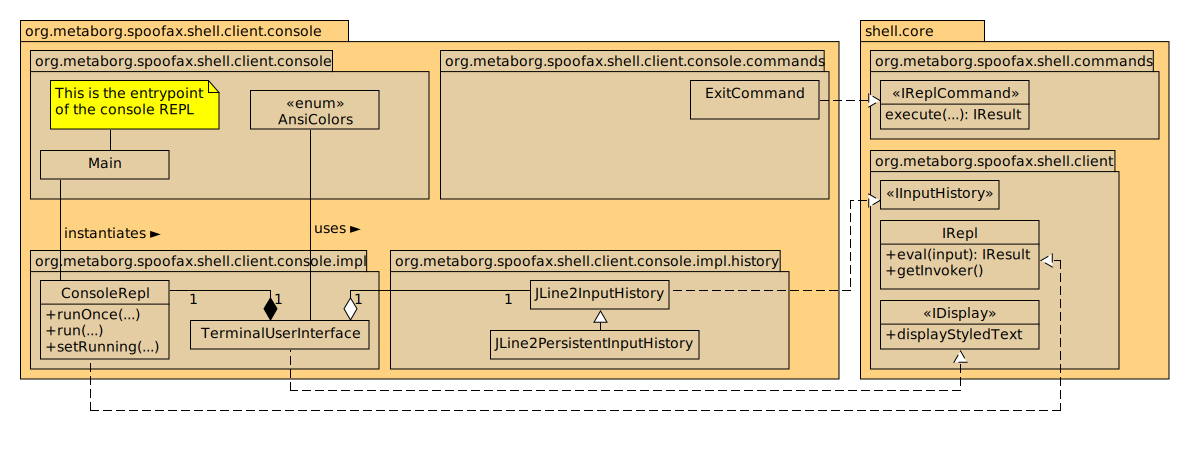
\includegraphics[width=\textwidth]{uml-console}
  \caption{UML diagram for the console frontend.}
  \label{fig:uml-console}
\end{figure}

As can be seen in \cref{fig:uml-console}, a frontend has to implement only a few
interfaces. The \texttt{ConsoleRepl} class is the central element in the
console frontend. It is instantiated first and controls the lifecycle of this
frontend. Its \texttt{run} method maps to the \texttt{loop} step in
Read-Eval-Print Loop and thus contains the \texttt{read}, \texttt{eval} and
\texttt{print} steps.

The \texttt{read} and \texttt{print} steps are provided
the by \texttt{TerminalUserInterface} class, which, as the name implies, is
responsible for the user interface. This class has connections to the standard
input, output and error streams. It uses JLine2 to provide a blocking input
editor. Because the input editor is blocking, the console frontend can run in a
single thread, thereby greatly simplifying its implementation.

A straightforward algorithm to provide multiline editing capabilities is used in
combination with JLine2's input buffer, which JLine2 does not natively support.
JLine2 does support input history, which means only an adapter class,
\texttt{JLine2InputHistory} had to be made to interoperate with the history
interface that is offered by the backend. An extension to this class is provided
to maintain persistent history.

To provide syntax and error highlighting, ANSI color codes are used. These
color codes are obtained through the \texttt{AnsiColors} enumeration, which
maps colors as returned by the \texttt{IResult} interface to their closest
ANSI equivalent.

Lastly, an \texttt{ExitCommand} is provided to halt the \texttt{run} method
in \texttt{ConsoleRepl}.

\subsection{Eclipse plugin}
\label{ssec:eclipse-plugin}

Spoofax currently features extensive integration in the Eclipse IDE. The client
expressed their interest to have this same level of integration for the REPL. A
plugin to the Eclipse IDE has been developed, which exposes the REPL
functionality through a graphical user interface that is familiar to anyone
working in Eclipse.

As is customary for a graphical user interface toolkit, the toolkit offered by
Eclipse uses multiple threads. One such thread is designated the ``UI thread'',
or user interface thread. This thread is responsible for processing
user-generated events (such as mouse clicks) and updating the graphical
representation of the widgets. All tasks that perform long running
calculations are supposed to be run in a background thread, such that the UI
thread is free to process incoming events. Instead, if a long running
computation is run in the UI thread, the widgets on the screen stop responding
to the user and the program appears to be in a frozen state. For this reason,
the backend has to perform its evaluations in a background thread, whilst all
the widgets and user interaction takes place in the UI thread.
The following discussion refers to the UML as depicted in
\cref{fig:uml-eclipse}.

\begin{figure}[h]
  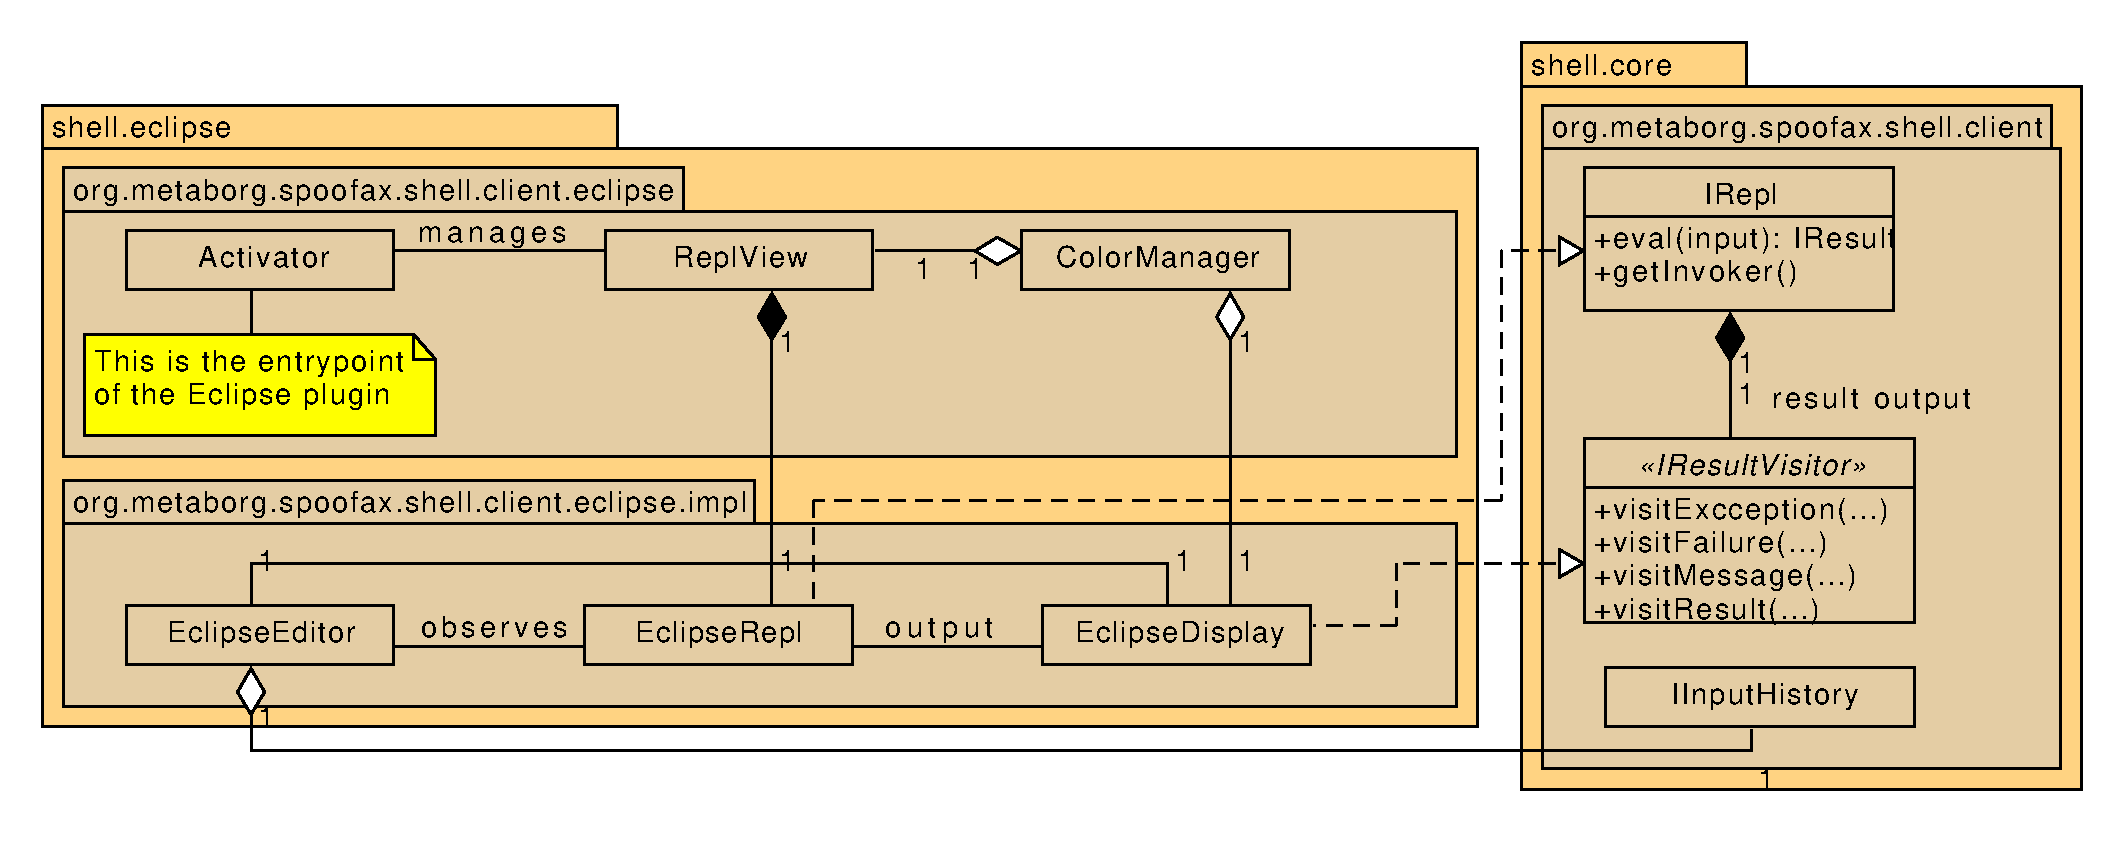
\includegraphics[width=\textwidth]{uml-eclipse}
  \caption{UML diagram for the Eclipse plugin.}
  \label{fig:uml-eclipse}
\end{figure}

Again, as can be seen in the UML, only a few interfaces have to be implemented.
The \texttt{EclipseRepl} class is the central element in the Eclipse plugin.
It is instantiated by the \texttt{ReplView} class, which in turn is
instantiated by Eclipse when the user requests the REPL to be opened. This
\texttt{ReplView} class also instantiates the input editor widget,
\texttt{EclipseEditor} and the \texttt{IResultVisitor} implementation,
\texttt{EclipseDisplay}.
In a multithreaded graphical user interface environment, asking text entry
widgets for the entered text is rarely a blocking process. This is no different
in Eclipse. For this reason, the \texttt{EclipseRepl} cannot simply loop as the
console frontend does. The solution is to use reactive programming through RxJava:
the \texttt{EclipseRepl} is registered as an observer to the
\texttt{EclipseEditor}. Then, when the user presses the Return key,
\texttt{EclipseEditor} notifies \texttt{EclipseRepl} with the contents of its
text buffer. \texttt{EclipseRepl} in turn launches a background job in which the
evaluation takes place, so as to not block the UI thread. Since the backend
simply returns an implementation of the \texttt{IResult} interface (see
\cref{sec:visitor}), the \texttt{EclipseRepl} can schedule the processing of this
result by the \texttt{EclipseDisplay} class on the UI thread. This processing
has to be done on the UI thread, because otherwise the \texttt{EclipseDisplay}
cannot update the widget it maintains to display results.
As one can see, the Eclipse plugin does not implement the \texttt{loop} step of
a REPL. There is no need to do so, due to the use of multithreading and reactive
programming.

%%% Local Variables:
%%% mode: latex
%%% TeX-master: "../main"
%%% End:
